\documentclass[11pt]{article}

\usepackage{paralist}
\usepackage{amsmath}
\usepackage{textcomp}
\usepackage[top=0.8in, bottom=0.8in, left=0.8in, right=0.8in]{geometry}
% add other packages here
\usepackage{courier}
\usepackage{graphicx}
\usepackage{array}
\usepackage{wrapfig}
% put your group number and names in the author field
\title{\bf Exercise 2: A Reactive Agent for the Pickup and Delivery Problem}
\author{Group \textnumero76: Simon Honigmann, Arthur Gassner}

% the report should not be longer than 3 pages

\begin{document}
\maketitle
\section{Problem Representation}

\subsection{Representation Description}
% describe how you design the state representation, the possible actions, the reward table and the probability transition table

Defining the states required considerable forethought, which took the form of a small scale notebook simulation. We first used only 3 cities, arranged in a triangle, to determine what information the agent would require to make an optimal decision. Using this method, we decided to structure the states and actions as follows. The agent's state is defined by it's current city and the destination city of any task (plus one case where there is no available task). To simplify the structure of our state transition table, we included entries for impossible states (e.g. having a task destination be the same city as the current city) and simply assigned a zero probability to these states. For N cities each with N+1 possible destinations (including no destination), this yields (N)x(N+1) possible states. Similarly, each state has a possible action. Again to simplify the logic, we defined one action for each city, that would represent ignoring any available tasks and proceeding to a given city, and one additional action for taking the available task.\\

Once the structure of the states and actions were defined, we created rules that could be used to generate the state transition probabilities. Based on our small scale test, we defined the following rules:
\begin{compactenum} 
	\item The task destination cannot equal the origin city. This applies to both present state (s) and future state (s'). 
	\item The present origin city cannot equal the future state's origin city (i.e. the agent must change cities every step of the simulation). 
	\item Regarding tasks:
	\begin{compactenum}
		\item If the task is accepted by the agent, the current destination city must equal the future state's origin city.  
		\item In all other cases:
		\begin{compactenum}
			\item the action cannot equal the current origin city and,
			\item the future origin city must equal the action city.
		\end{compactenum}
	\end{compactenum}		
	\item All matrix entries that satisfy all above conditions are to be populated as follows:
	\begin{compactenum}
		\item If the future state has a task available, then the probability is $ T(s,a,s')=p(s'_{origin},s'_{destination}) $ where $p$ is the task probability distribution defined in the xml document. 
		\item If the future state has no task available, the probability is $T(s,a,s')=1-\sum p(s'_{origin},s'_{i}) $ where i indexes all cities. 
	\end{compactenum}
\end{compactenum}
For all cases that were defined as impossible by the rule set, a zero probability was assigned.\\

Defining the expected rewards, denoted "Profit" in our code was easy enough. For each of (N)(N+1) states and (N+1) actions, the profit was defined as follows: 
\begin{itemize}
	\item If the agent takes an available task, then Profit equals \\ 
	$ P(s,a)=r(s_{origin},s_{destination})-c(s_{origin},s_{destination}) $
	\item Else if the agent decides instead to go to an adjacent city, then Profit simply equals:\\ $P(s,a)=-c(s_{origin},a_{destination}) $
\end{itemize}
Where $P(s,a)$ denotes the profit for a given state, s, and action, a, and $r(origin,destination)$ and $c(origin,destination)$ each represent the respective delivery reward and cost of travel between two cities. Cost of travel was defined as the travel distance multiplied by a constant cost-per-distance. We defined the cost-per-distance to be one for all experiments.\\

To test our created tables, we manually reviewed the generated matrix, and tested the central and boundary cases for correctness. Checks were repeated for all provided city .xml files to ensure the robustness of the algorithms. Once satisfied with our results, we proceeded to developing an off-line reinforcement learning algorithm for the agents. 

\subsection{Implementation Details}
% describe the implementation details of the representations above and the implementation details of the reinforcement learning algorithm you implemented
Despite vehicles only being able to travel to directly adjacent cities, agents are allowed to decide to move to any city if it the decision algorithm indicates it is the best decision. However, when the agent reaches an intermediary city, the agent is still able to re-evaluate the decision based on the actual state reached. For instance, if the intermediary city has an improbable yet valuable task available, the agent could change course and accept the task. \\

To compute the best action, $Best(s)$ for each possible state, an iterative optimization algorithm was is computed at the start of each simulation. For each starting state, every action was considered and the reward for that action was determined using the previously determined Profit matrix. Then, to consider future possibilities leading from the resulting state, for each possible future state, the state transition probability was multiplied by the max value of the future state, $V(s')$, and discounted by a factor $\gamma$. The max possible value, $V(s)$, for all actions value is stored, and then serves as the baseline for the next iteration of calculations. Once the max value converges (due to the discount factor), the best action is set to be the action leading to the max value. \\

All mentioned tables and matrices were structured as nested ArrayLists so that memory could be dynamically allocated when different .xml files are used. By looping through all possible index combinations and applying the conditions above, the tables could be initialized with values. Again, all possible states and actions were considered and the best action and maximum values were saved in nested ArrayLists for future use. 

\section{Results}
% in this section, you describe several results from the experiments with your reactive agent
The simulation was tested thoroughly with different conditions to better understand value of using offline reinforcement learning algorithms, and the importance of different discount factors. 
\subsection{Experiment 1: Discount factor}
% the purpose of this experiment is to understand how the discount factor influences the result
\begin{wrapfigure}{R}{0.5\textwidth}
	\centering
	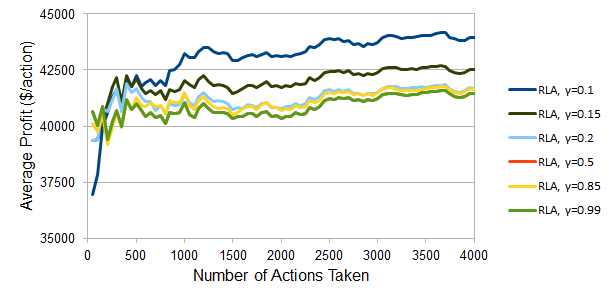
\includegraphics[width=0.5\textwidth]{p1}
	\caption{Average profit for 6 agents with different discount factors traveling in The Netherlands}
	\label{figure:1}
\end{wrapfigure}
\subsubsection{Setting}
% you describe how you perform the experiment (you also need to specify the configuration used for the experiment)
The first experiment investigates the short-term and long-term value of different discount factors.\\

In order to do that, we ran 6 separate simulations with the following discount rates : 0.1, 0.15, 0.2, 0.5, 0.85 and 0.99.\\

Each simulation used the configuration specified by the \texttt{reactive2.xml} file.\\

We recorded the average profit of each agent every 50 actions, until the 4000th action had been made and plotted the result (see Figure 1).\\


\subsubsection{Observations}
As we can see in Figure 1, once enough actions have been made, the average profit of each agent settles around a certain value.\\

Another important observation is how the variation of the discount factor influences the average profit. There's barely any change for a discount factors ranging from 0.2 to 0.99. But once we use a discount factor of 0.2 and below, the "settling value" of the average profit increases in a quicker fashion.\\
% you describe the experimental results and the conclusions you inferred from these results

\subsection{Experiment 2: Comparisons with dummy agents}
% you compare the results of your agent with two dummy agents: the random agent that was already given in the starter files and another dummy agent that you define and create. You should report the results from the simulations using the topologies given in the starter files and optionally, additional topologies that you create
\begin{wrapfigure}{R}{0.5\textwidth}
	\centering
	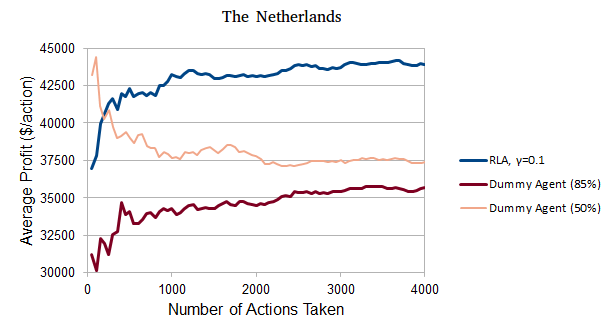
\includegraphics[width=0.5\textwidth]{p21}
	\caption{Average profit of our RLA agent and two dummy agents in four different countries}
	\label{figure:1}
\end{wrapfigure}
\subsubsection{Setting}
% you describe how you perform the experiment and you describe the dummy agent you created (you also need to specify the configuration used for the experiment)
The second experiment investigates how RLA trained agents' average profits compared to dummy agents' average profit.\\


To simulate the dummy agents, we used the \texttt{ReactiveTemplate.java} provided. We used the two dummy agents specified in \texttt{agents.xml} : \texttt{reactive-random} and \texttt{reactive-random-50}.\\

We ran each simulation for the four different topologies provided.\\

\subsubsection{Observations}
% elaborate on the observed results
We can see that the RLA trained agent performs better than both dummy agents.\\

Secondly, the

\end{document}